\documentclass[11pt]{article}
\usepackage[utf8]{inputenc}
\usepackage[T1]{fontenc}
\usepackage[spanish, es-noshorthands,activeacute]{babel}
\usepackage[pdftex,usenames,dvipsnames]{color}
\usepackage{amsmath}
\usepackage{amssymb}
%\usepackage{mathpazo}
%\usepackage{color}
\usepackage{fancyhdr}
\usepackage{graphicx}
\graphicspath{ {./ImgsPr4/} }
\usepackage{wrapfig}
\usepackage{whilecode2}
%\usepackage[shortlabels]{enumitem}
%\usepackage{bm}
%\usepackage{lastpage}
%\usepackage{enumitem}
\usepackage{subcaption}
\usepackage{graphicx}
\DeclareCaptionFormat{custom}
{%
    \textbf{#1#2}\textit{\small #3}
}
\captionsetup{format=custom, labelformat=empty}


\parindent=5mm
\renewcommand*{\baselinestretch}{1}
\parskip=1mm
\voffset=-10.4mm
\hoffset=-10.4mm
\oddsidemargin=0mm
\topmargin=0mm
\headheight=4.579965mm
\headsep=3.420035mm
\textwidth=180mm
\textheight=251mm
\marginparsep=0mm
\marginparwidth=0mm
\footskip=8mm
\paperwidth=210mm
\paperheight=297mm

\newcounter{exercise}[section]
\newenvironment{exercise}[2][]{\refstepcounter{exercise}\par\medskip
\noindent \textbf{Exercise~\theexercise.  #2\newline} \rmfamily}{\medskip}

\newenvironment{exercise*}[2][]{\refstepcounter{exercise}\par\medskip
\noindent \textbf{Exercise~\theexercise.  #2\newline} \rmfamily}{\medskip}

\newenvironment{ejercicio}[2][]{\refstepcounter{exercise}\par
 \textbf{Ejercicio~\theexercise.  #2\newline} \rmfamily}{}

\newenvironment{apartado}[2][]{\refstepcounter{exercise}\par
 \textbf{Apartado~\theexercise.  #2\newline} }{}

\newenvironment{inlinedefinition}[2]
    {\begin{center}
    \begin{tabular}{p{0.9\textwidth}}
    
    \textit{\textbf{#1}.}
    }
    { 
    
    \end{tabular} 
    \end{center}
    }

\pagestyle{fancy}
\fancyhf{}
\lhead{\footnotesize{Teoría de Autómatas y Lenguajes Formales}}
\rhead{\footnotesize{Práctica IV}}
\lfoot{\footnotesize{Carlos Martínez Zurita}}
\rfoot{\footnotesize{\thepage}}
\renewcommand{\footrulewidth}{1pt}
\renewcommand{\headrulewidth}{1pt}
\begin{document}
	\medskip \sffamily \Large{\centerline{\textbf{Práctica IV: Codificación de vectores y programas WHILE en Octave}}}\large{\centerline{\textbf{Teoría de Autómatas y Lenguajes Formales}}}\rmfamily\normalsize
	\begin{ejercicio}{Cree el programa WHILE más simple que calcule la función "diverge" (con cero argumentos)}
	\par{\whileprogram{diverge}{0}{
		\DefaultVar{2}\Assig\Inc{\DefaultVar{1}} \Comment{Nos aseguramos de que $X_2\neq 0$}		
		\While{\DefaultVar{2} \not = 0} {\Comment{Bucle infinito}
			\DefaultVar{1}\Assig 0
		}
	}{s}}
	\par{Podemos comprobar en Octave que su codificación es: }
	\begin{figure}[h]
	    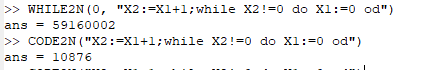
\includegraphics[width=0.5\textwidth]{divergeEncoding}
	    \caption{Codificación mínima de la función "diverge"}
	    \label{fig:diverge}
	\end{figure}
	}
	\end{ejercicio}
	\begin{ejercicio}{Describe en Octave una función que enumere todos los vectores de cualquier dimensión}
	\par{Ya tenemos un script que devuelve el vector asociado a un número natural. Esto simplifica mucho las cosas, ya que podemos usarlo para obtener todos los vectores: $godelencoding(1), godelencoding(2),\dots$. $godelencoding$ está definido en los apuntes como $\gamma$, cuyo segundo argumento define la componente del vector que queremos devolver. Definimos, pues, la función $godelall: \mathbb{N}\rightarrow P(\mathbb{N}^*)$ que, dado un natural (o el 0), devuelve los vectores asociados a todos los naturales hasta ese número. Nótese que la función no es sobreyectiva, ya que $|P(\mathbb{N}^*)|=\aleph_1\neq\aleph_0=|\mathbb{N}^*|$
	\begin{verbatim}
	function code=godelall(n)
  	encodings=["(",int2str(godeldecoding(0)),")"]
  	for i = 1:n
    		encodings=[encodings,", (",int2str(godeldecoding(i)),")"]
  	endfor
	end
	\end{verbatim}
	Podemos comprobar, al ejecutar y comparar en los apuntes, que el programa funciona:
	\begin{figure}[h]
	    \centering
	    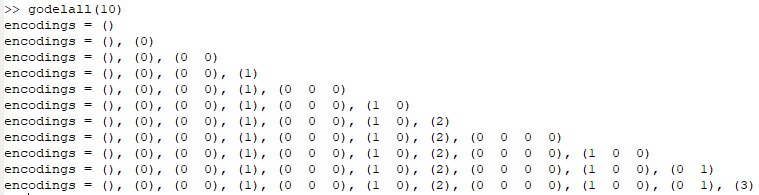
\includegraphics[width=0.8\textwidth]{godelAllExample}
	    \caption{Ejemplo exitoso de ejecución}
	    \label{fig:godelall}
	\end{figure}
	}
	\end{ejercicio}
	\begin{ejercicio}{Describe en Octave una función que enumere todos los programas WHILE}
	\par{Ya tenemos un script que devuelve el código WHILE asociado a un número natural. Esto simplifica mucho las cosas, ya que podemos usarlo  para devolver todos los programas WHILE: $N2WHILE(1), N2WHILE(2),\dots$. $N2WHILE$ está definido en los apuntes. Definimos, pues, la función $whileall: \mathbb{N}\rightarrow P(WHILE)$ que, dado un natural (o el 0), devuelve los programas asociados a todos los naturales hasta ese número. De nuevo, la función no es sobreyectiva.
	\begin{verbatim}
	function code=whileall(n)
	encodings=N2WHILE(0)
  	for i = 1:n
    		encodings=[encodings,"\n#######\n",N2WHILE(i)]
  	endfor
	end
	\end{verbatim}	
	Podemos usar esta función para comprobar que el ejercicio 1 está bien resuelto, introduciendo su codificación y viendo si antes de que aparezca nuestro programa,aparece otro que también diverja. En la práctica, no podemos hacer eso, ya que la codificación es un número muy alto.
	\begin{figure}[h]
	    \centering
	    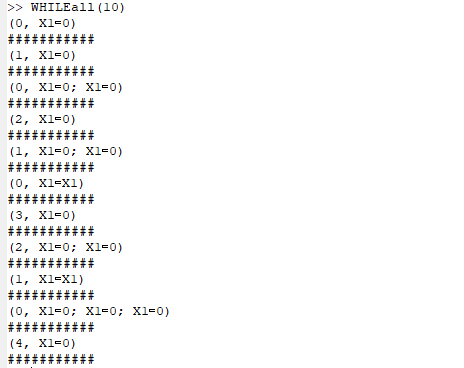
\includegraphics[width=0.7\textwidth]{whileAllExample}
	    \caption{Programas WHILE de codificación menor o igual que 10}
	    \label{fig:whileall}
	\end{figure}
	}
	}
	\end{ejercicio}
\end{document}